\section{Theoretical and Simulation Analysis}
\label{sec:analysis}

In order to compare \textit{side by side}, we'll discuss the theoretical and simulation analysis at the same time.

However, one has to present and analyse the two stages in order to fully understand the simulation. The constants values used are expressed in the table below.

\begin{table}[h]
    \centering
    \begin{tabular}{|l|c|c|}
    \hline
    {\bf Name} & {\bf Value} & {\bf Units} \\ \hline
    $R_1$ & $33.7$ & $k\Omega$ [kOhms] \\ \hline
    $R_2$ & $3.6$ & $k\Omega$ [kOhms] \\ \hline
    $R_C$ & $3.8$ & $k\Omega$ [kOhms] \\ \hline
    $R_E$ & $200$ & $\Omega$ [Ohms] \\ \hline
    $R_{out}$ & $400$ & $\Omega$ [Ohms] \\ \hline
    $C_{in}$ & $800$ & $\mu F$ [$\mu$Farads]\\ \hline
    $C_E$ & $800$ & $\mu F$ [$\mu$Farads] \\ \hline
    $C_o$ & $600$ & $\mu F$ [$\mu$Farads] \\ \hline
    \end{tabular}
    \caption{Constants Values}
    \label{tab:constants}
\end{table}

\subsection{Gain Stage}
\label{subsec:stat}

Firstly, we must discuss the first half of the circuit that was used. Its goal is to ensure a high input voltage so the input signal is not degradated or distorted throughout the circuit. It also has an elevated gain associated, so this is the part that is responsible for the signal amplification.

A scheme of this circuit is presented below.

\begin{figure}[h]
    \centering
    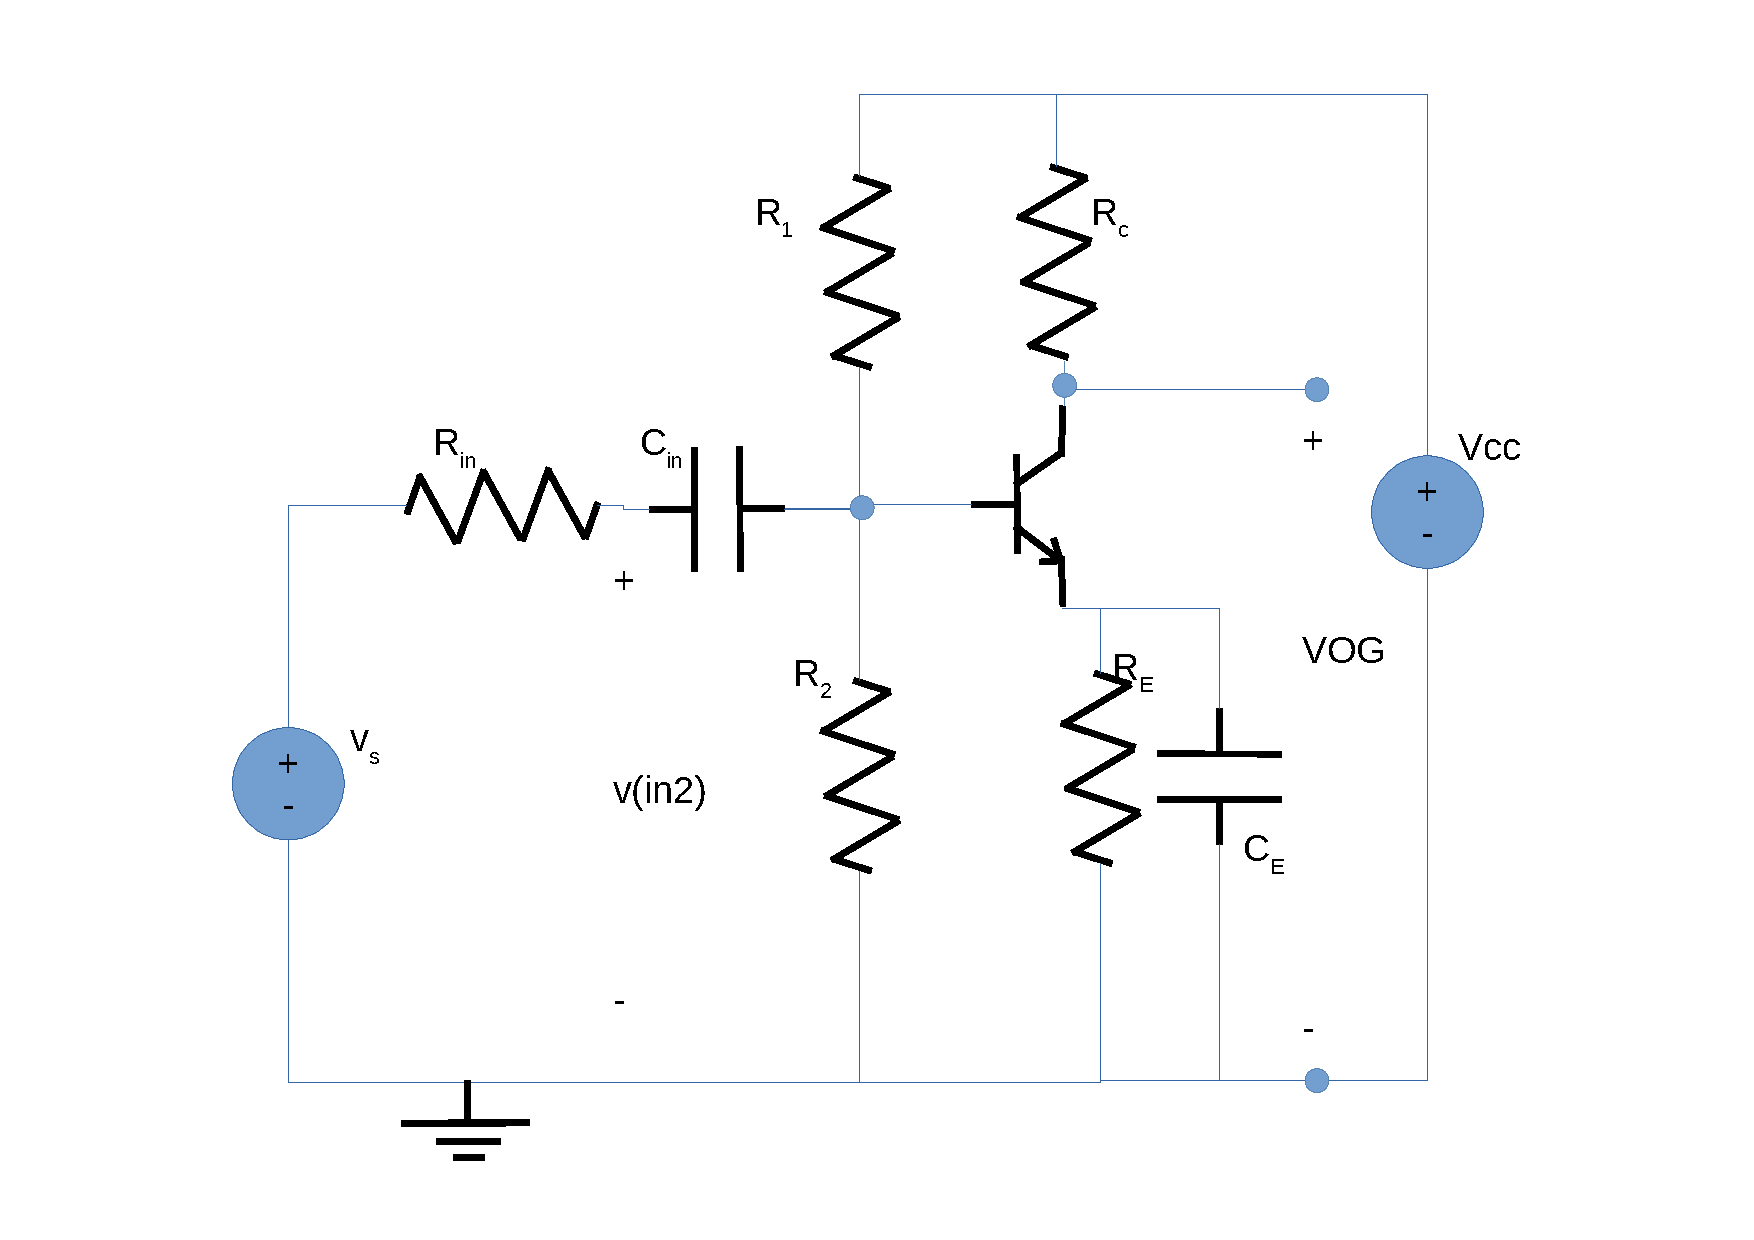
\includegraphics[scale=0.4]{gain_stage_l4.pdf}
    \caption{Gain Stage}
    \label{fig:gain_stage}
\end{figure}

As one can see, there are 3 types of elements: a NPN BJT, resistors and capacitors.

The first capacitor, $C_{in}$, is a coupling capacitor, as it acts as a DC Block, so that $V_{in}$ doesn't impose a DC component of 0, that would change the OP of the transistor.

The second capacitor, $C_E$, acts as a bypass capacitor, for it ensures that for low frequencies all the current flows through $R_E$, and for high frequencies, it passes through the capacitor.

Generally, the output impedance of this stage ($Z_{O1}$) is high, when compared with the load, being the major reason why one cannot use just this stage, and we need another one.

\subsection{Output Stage}

As we could see in the previous section, the Gain Stage has a high $Z_{O1}$. For that reason, we connect a second circuit to the output of the Gain Stage, that presents a low output impedance.

A scheme of this stage is presented below, 

\begin{figure}[h]
    \centering
    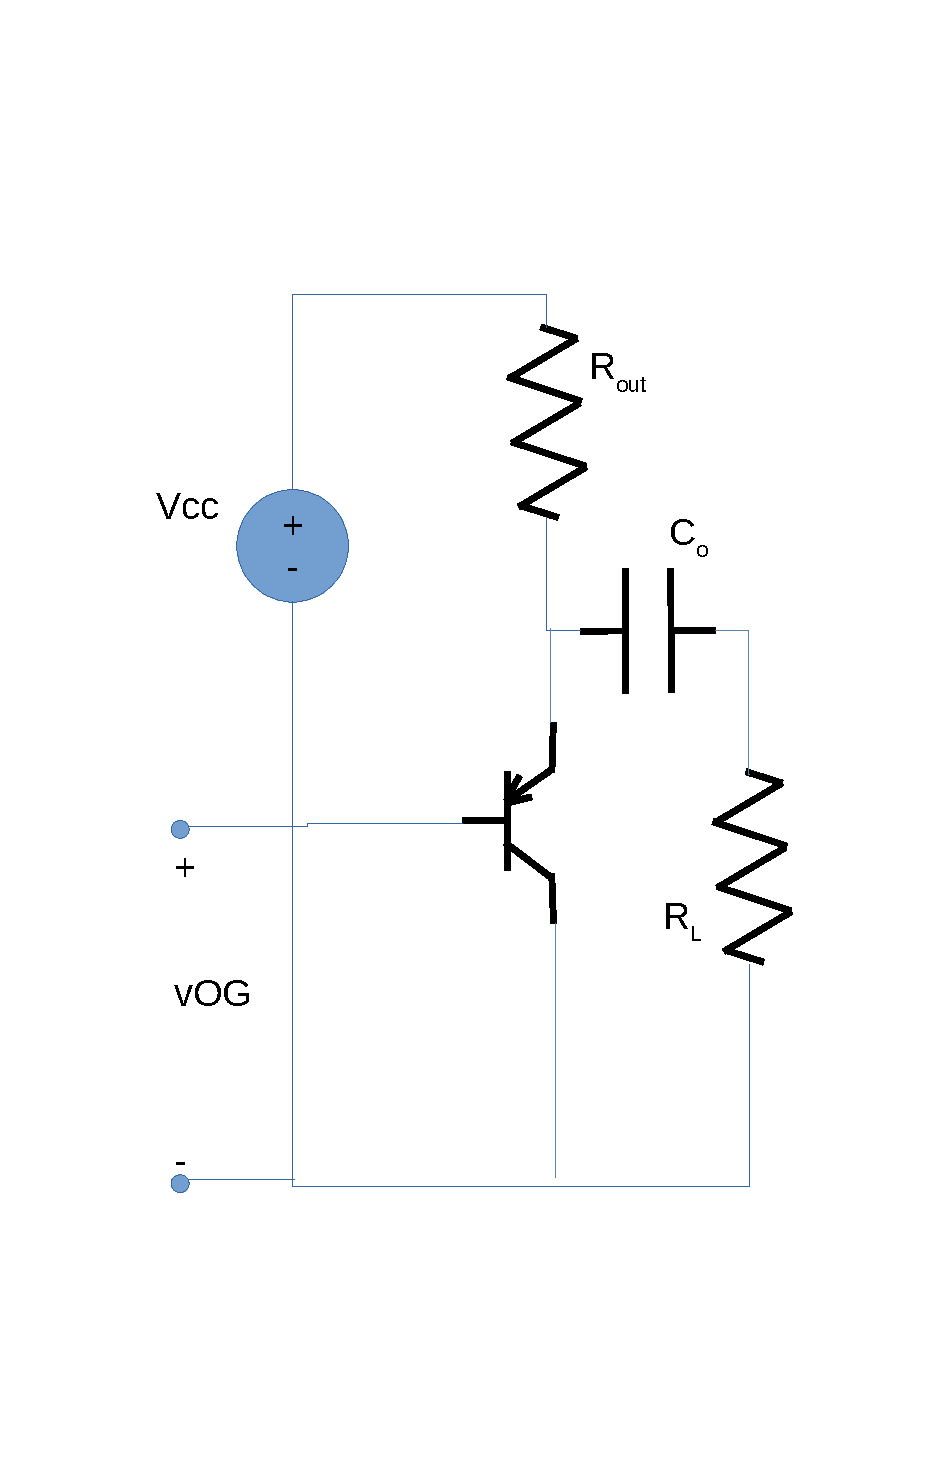
\includegraphics[scale=0.5]{output_stage_l4.pdf}
    \caption{Output Stage}
    \label{fig:regulator}
\end{figure}

As one can see, this circuit presents similar components, however, with mild differences.

Instead of a NPN BJT, we use a PNP BJT, because it has a higher $\beta_F$, which lowers the output impedance (which is what we want). Besides, it illustrates the use of another BJT transistor.

Another capacitor, $C_o$, is used with a similar goal as the previous coupling capacitor. If we didn't use such component, the gain stage would impose a DC voltage of 0 to the second stage, which would ruin the transistor's OP. 

As we'll see, we end up with a lower output impedance in this stage (when compared to the load) and a higher input impedance (when compared to the output impedance of the gain stage).

When combining both stages, we need to ensure that there is a compatibility  between the impedances. In fact, by the voltage divider law, to make sure no voltage signal is lost, the input impedance of the second stage should be much greater than the output impedance of the first one. 

In conclusion, when we merge these two circuits, we end up with our BJT Amplifier as seen in Figure \ref{fig:circuitol4}.

\clearpage
\subsection{Theoretical Analysis}
\label{subsec:Req}

\subsubsection{Impedances}

On the Theoretical side, we will evaluate the four impedances associated with the two stages ($Z_{I1}, Z_{O1}, Z_{I2}$ and $Z_{O2}$) as well as the two gains associated with each stage ($A_{V1}$ and $A_{V2}$).
To do so, we need to perform an Operating Point Analysis to find the values necessary for the Incremental Analysis.

Regarding the first stage (Gain Stage), the input and output impedances (\{$Z_{I1}$, $Z_{O1}$\}, respectively) can be derived by KVL and KCL, leading us to the following expressions:

\begin{equation}
    Z_{I1}=R_B // r_{\pi 1}
\end{equation}
where $R_B=R_1 // R_2$.

Because of the presence of the bypass capacitor and also because in this theorectical approach it is assumed the capacitors are short-circuited (high-frequency analysis), $R_E \simeq 0$. This first stage input impedance matches also with the total input impedance of the circuit, as this stage is load-independent.

On the other hand, the first stage output impedance can be obtained by:

\begin{equation}
    Z_{O1}=r_o // R_C  
\end{equation}

Regarding the second stage, by analysing the circuit we get:

\begin{equation}
    Z_{I2}=\frac{(g_{m2}+g_{\pi2}+g_{o2}+g_{E2})}{g_{\pi2}(g_{\pi2}+g_{o2}+g_{E2})}
\end{equation}

\begin{equation}
    Z_{O2}=\frac{1}{(g_{m2}+g_{\pi2}+g_{o2}+g_{E2})}
\end{equation}

And finally, the total output impedance:

\begin{equation}
    Z_{OT}=\frac{v_o}{i_o}=\frac{1}{g_{o2}+g_{m2}\frac{r_{\pi2}}{r_{\pi2}+Z_{O1}}+g_{E2}+\frac{1}{r_{\pi2}+Z_{O1}}}
\end{equation}

The 4 values are presented below,

\begin{table}[h]
    \centering
    \begin{tabular}{|l|c|}
    \hline
    {\bf Impedances} & {\bf Ohms ($\Omega$)} \\ \hline
    Z1_I	&	32258.268036\\\hline
Z1_O	&	942.142024\\\hline
Z2_I	&	8598.855359\\\hline
Z2_O	&	0.302173\\\hline

    \end{tabular}
    \caption{Theoretical Impedances}
    \label{tab:theo_imp}
\end{table}

As a result of the compromise between the cost and overall performance, the total output impedance was unpurposely sacrified, which is of course not what we would desire (especially because the speaker impedance is 8 $\Omega$). 

As one can see, regarding the compatibility between both stages (remembering that $Z_{O1}$ needs to be  much lower than $Z_{I2}$), we have pretty satisfactory results. This is needed so that there is no signal degradation or loss between these stages. It's clear that $V_{in2}$ needs to be as close as possible to $V_{O2}$, confirmed if we apply a voltage divider with $Z_{I2}>>Z_{O1}$:

\begin{equation}
    V_{in2} = \frac{Z_{I2}}{Z_{I2}+Z_{O1}} V_{O2}. 
\end{equation}

\subsubsection{Gain}

In order to calculate the total gain ($A_{V}$) we performed a simple multiplication, so that we have $A_V=A_{V1}A_{V2}$. Although being an approximation, the real interaction between both stages is negligible, and because of that we can compute the gain as if it was the total gain of both separate stages.

We present a compilation of the values below,


\begin{table}[h]
\parbox{.4\linewidth}{
  \centering
    \begin{tabular}{|l|c|}
    \hline
    {\bf Gain} & {\bf Value} \\ \hline
    $G_1$	&	-264.565721\\\hline
$G_2$	&	0.991532\\\hline
$G_T$	&	-252.275561\\\hline
$G_{T_{dB}}$	&	48.037504\\\hline

    \end{tabular}
    \caption{Theoretical upper gain bound results}
    \label{tab:theo_gains_high}
  }
  \hfill
  \parbox{.4\textwidth}{
  \centering  
  \begin{tabular}{|c|c|}
    \hline    
    {\bf Gain} & {\bf Value} \\ \hline
    $G_1$	&	-17.126226\\\hline
$G_2$	&	0.991532\\\hline
$G_T$	&	-16.330643\\\hline
$G_{T_{dB}}$	&	24.260066\\\hline

  \end{tabular}
  \caption{Theoretical lower gain bound results}
  \label{tab:theo_gains_low}
  }
  \end{table}
  
Note that the first approximation considers $C_E$ to be short-circuited and the second one that $C_E$ behaves as an open circuit. The simulation results should bear within these two boundaries (as they actually do, see table \ref{tab:sim_results}) since the capacitor is never either \textit{SC} or \textit{OC}. These bounds as well as an approximation for the real gain will be plotted in Section \ref{subsec:comparison}.

In order to acquire a better comparison between theory and simulation, besides this aproach, that considers the gain to be constant through all the frequencies , we also performed the \textit{Time constant method} for the lower cut-off frequency.

We calculate the lower cut-off frequency ($\omega_L=2\pi f_{CO_L}$) as,

\begin{equation}
    \omega_L=1/{R_{eq_i}C_i} + 1/{R_{eq_e}C_e} + 1/{R_{eq_o}C_o}
    \implies f_{CO_L}=2\pi w_L
\end{equation}

where $R_{eq}\equiv$ equivalent resistor as seen by each capacitor when the others are short-circuits.

We have,

\begin{equation}
    R_{eq_{in}} = R_{in}+Z_{I1}
\end{equation}

\begin{equation}
    R_{eq_e} = R_E // (\frac{1}{\frac{1}{R_s||R_B+r_{\pi}}+\frac{g_m r_{\pi}}{R_s||R_B+r_{\pi}}}) \simeq R_E//(\frac{r_{\pi}+R_s||R_B}{r_{\pi}}\frac{1}{g_m}) \simeq 1/g_{m}
\end{equation}

\begin{equation}
    R_{eq_o}=R_L+Z_{O}
\end{equation}

One could also do the reciprocal, but with the capacitors as open circuits in order to determine the higher cut-off frequency.
Like that, we just have to consider as approximation, a slope of $+20dB/dec$, until $f_{CO_L}$ is reached (which gives a better approximation than the constant gain one).

The theoretical value of the lower cut-off frequency is presented in the table below and will be better analysed and compared in Section \ref{subsec:comparison}.

\begin{table}[h]
    \centering
    \begin{tabular}{|l|c|}
    \hline
    {\bf Name} & {\bf Value [Hz]} \\ \hline
    Lower CO freq	&	28.296662\\\hline

    \end{tabular}
    \caption{Theoretical Lower Cut-off frequency}
    \label{tab:theo_CO_freq}
\end{table}

\pagebreak

\subsection{Simulation Analysis}
\label{subsec:Req}

On the Simulation Side, we are interested in the two impedances associated with the circuit as a whole ($Z_I$ and $Z_O$), both cut-off frequencies ($f_{CO_L}$ and $f_{CO_H}$), the bandwidth (interval between the cut-off frequencies) and the total gain ($A_V$) measured in the bandpass region. The measurement of these parameters and the overall performance of the circuit is outlined in \ref{sec:merit}.

We also confirm whether the BJTs are on the Forward Active Region (FAR), by comparing $V_{CE}$ and $V_{BE}$ for the NPN (and, analogously, $V_{EC}$ and $V_{EB}$ for PNP). 

The confirmation is presented below:

\begin{table}[h]
    \centering
    \begin{tabular}{|c|c|}
    \hline
    {\bf Name} & {\bf Value} \\ \hline
    V_CE & 3.02156\\ \hline
V_BE & 0.708289\\ \hline
V_CE>V_BE & Yes\\ \hline

    \end{tabular}
    \caption{NPN voltages and FAR confirmation}
    \label{tab:NPN}
\end{table}

\begin{table}[h]
    \centering
    \begin{tabular}{|c|c|}
    \hline
    {\bf Name} & {\bf Value} \\ \hline
    V_CE & 4.70867\\ \hline
V_EB & 0.814475\\ \hline
V_EC>V_EB & Yes\\ \hline

    \end{tabular}
    \caption{PNP voltages and FAR confirmation}
    \label{tab:PNP}
\end{table}


Regarding the results obtained, we present them in the table below:

\begin{table}[h]
    \centering
    \begin{tabular}{|c|c|c|}
    \hline
    {\bf Name} & {\bf Value} & {\bf Units}\\ \hline
    V_Gain & 37.904\\ \hline
Bandwidth & 1.59486E+06\\ \hline
CO_Freq & 8880.42\\ \hline

    \end{tabular}
    \caption{Simulation results}
    \label{tab:sim_results}
\end{table}

These results are to be explained and compared to the theoretical approach further into the report. But as quick note, we can see, as previously mentioned, that the value of the Gain, in dB, is within the theoretical boundaries prediction.


\subsubsection{Coupling Capacitors}

The understanding of the Coupling Capacitors' behaviour is crucial in order to analyse this circuit. In our BJT amplifier circuit there are two coupling capacitors ($C_O$ and $C_{in}$) but, since their functions are analogous, we shall focus on the capacitor $C_{in}$.

Below, we present 2 figures of the frequency response analysis, just by changing the parameter $C_{in}$ in a drastical way.

\begin{figure}[h]
\centering
\begin{subfigure}{.5\textwidth}
    \centering
    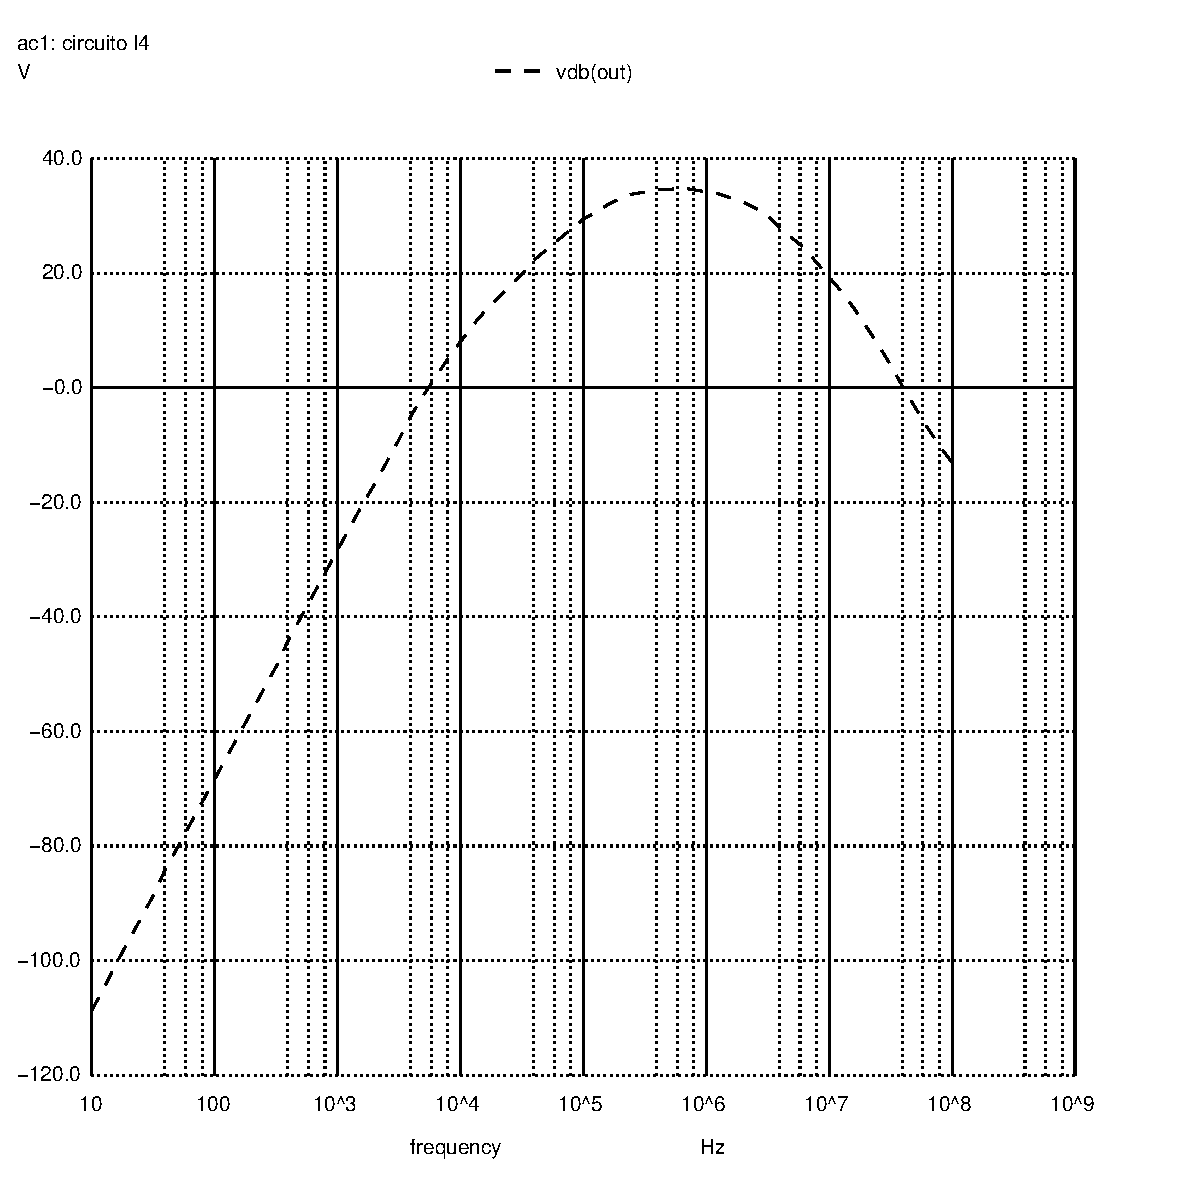
\includegraphics[scale=0.33]{images/cilow_1n.eps}
    \caption{$C_i$ low (1$nF$)}
\end{subfigure}%
\begin{subfigure}{.5\textwidth}
    \centering
    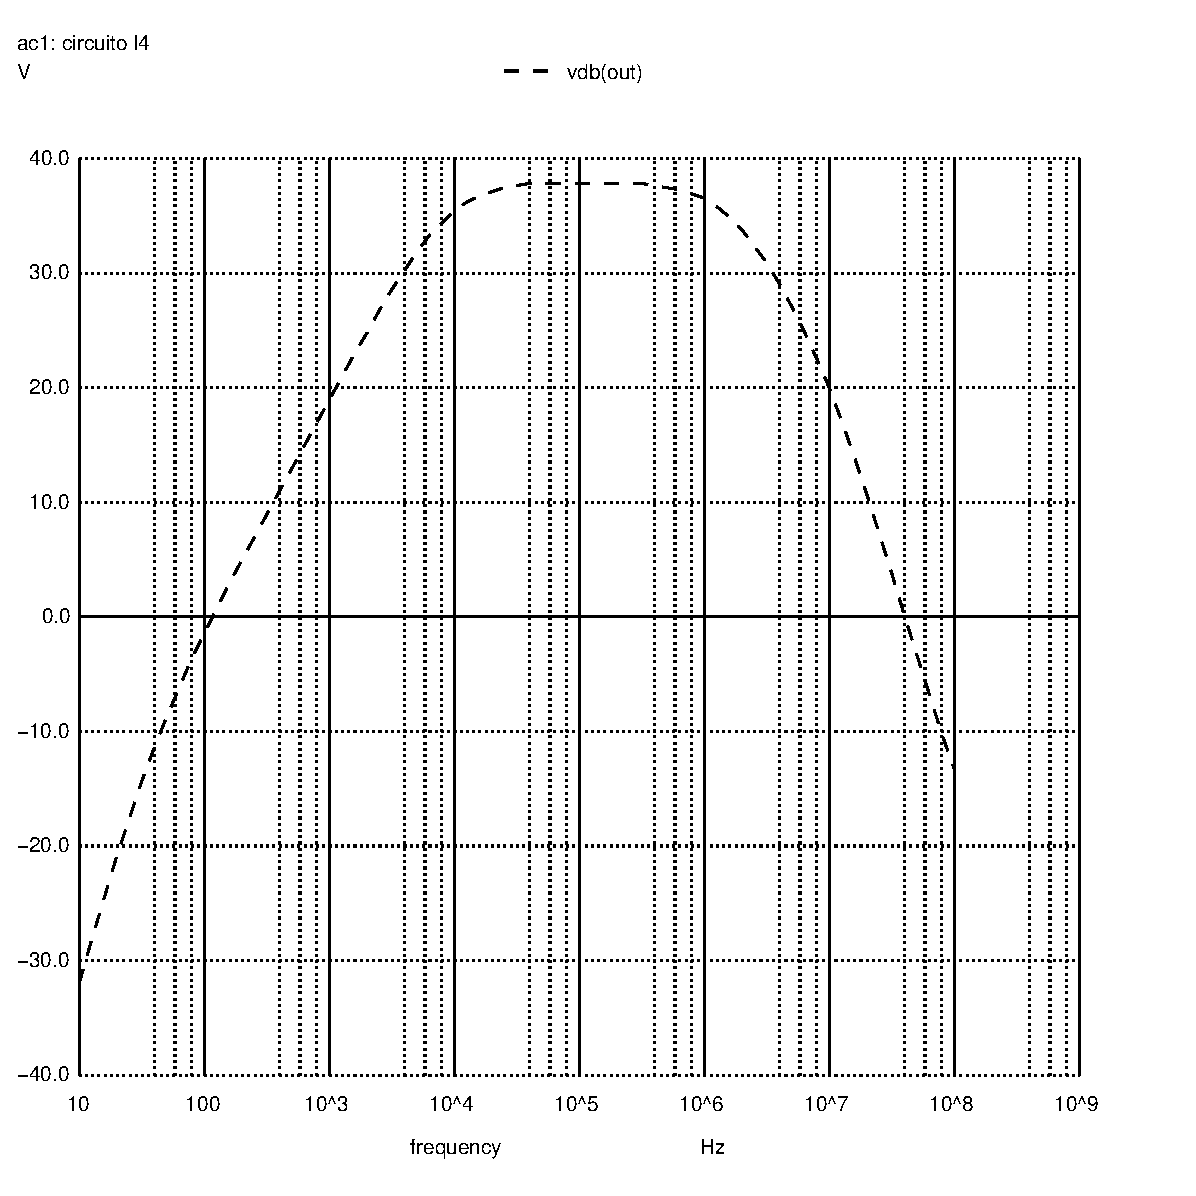
\includegraphics[scale=0.33]{images/cihigh_1.eps}
    \caption{$C_i$ high (1$F$)}
\end{subfigure}
\caption{$C_{in}$ influence}
\end{figure}

\pagebreak

As one can realise, the increase of the capacitance \textit{pushes} the cutoff frequency to the left, anticipating it, without changing the higher cut-off frequency, which leads to a larger bandwidth (desired).

This is not surprising because, as discussed previously, as $\omega \to 0$, $Z(C_{in}) \to \inf$, so this capacitor prevents the transistor from entering on either the saturation or cut-off regions, by blocking the DC component of the AUDIO IN source, as previously discussed. This helps mantaining the OP of the transistor, so that it can operate at lower frequencies, as $C_{in}$ increases.

\subsubsection{Bypass Capacitor}

Below, we present 2 figures of the frequency response analysis, just by changing the parameter $C_E$.

\begin{figure}[h]
\centering
\begin{subfigure}{.5\textwidth}
    \centering
    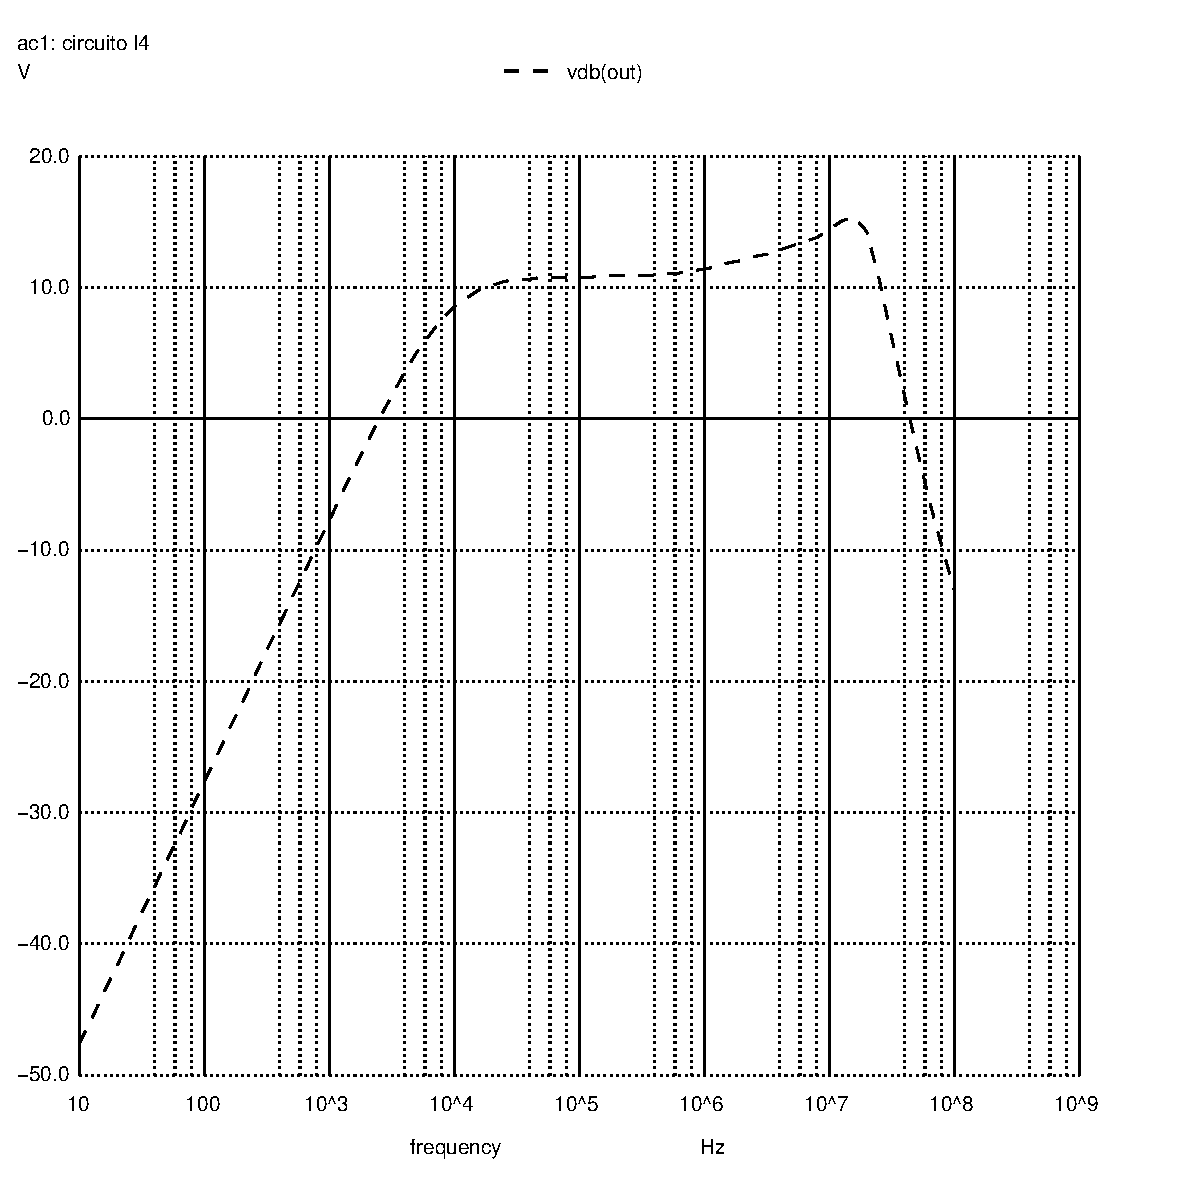
\includegraphics[scale=0.33]{images/celow_1n.eps}
    \caption{Low $C_E$ effect on Gain (1$nF$)}
\end{subfigure}%
\begin{subfigure}{.5\textwidth}
    \centering
    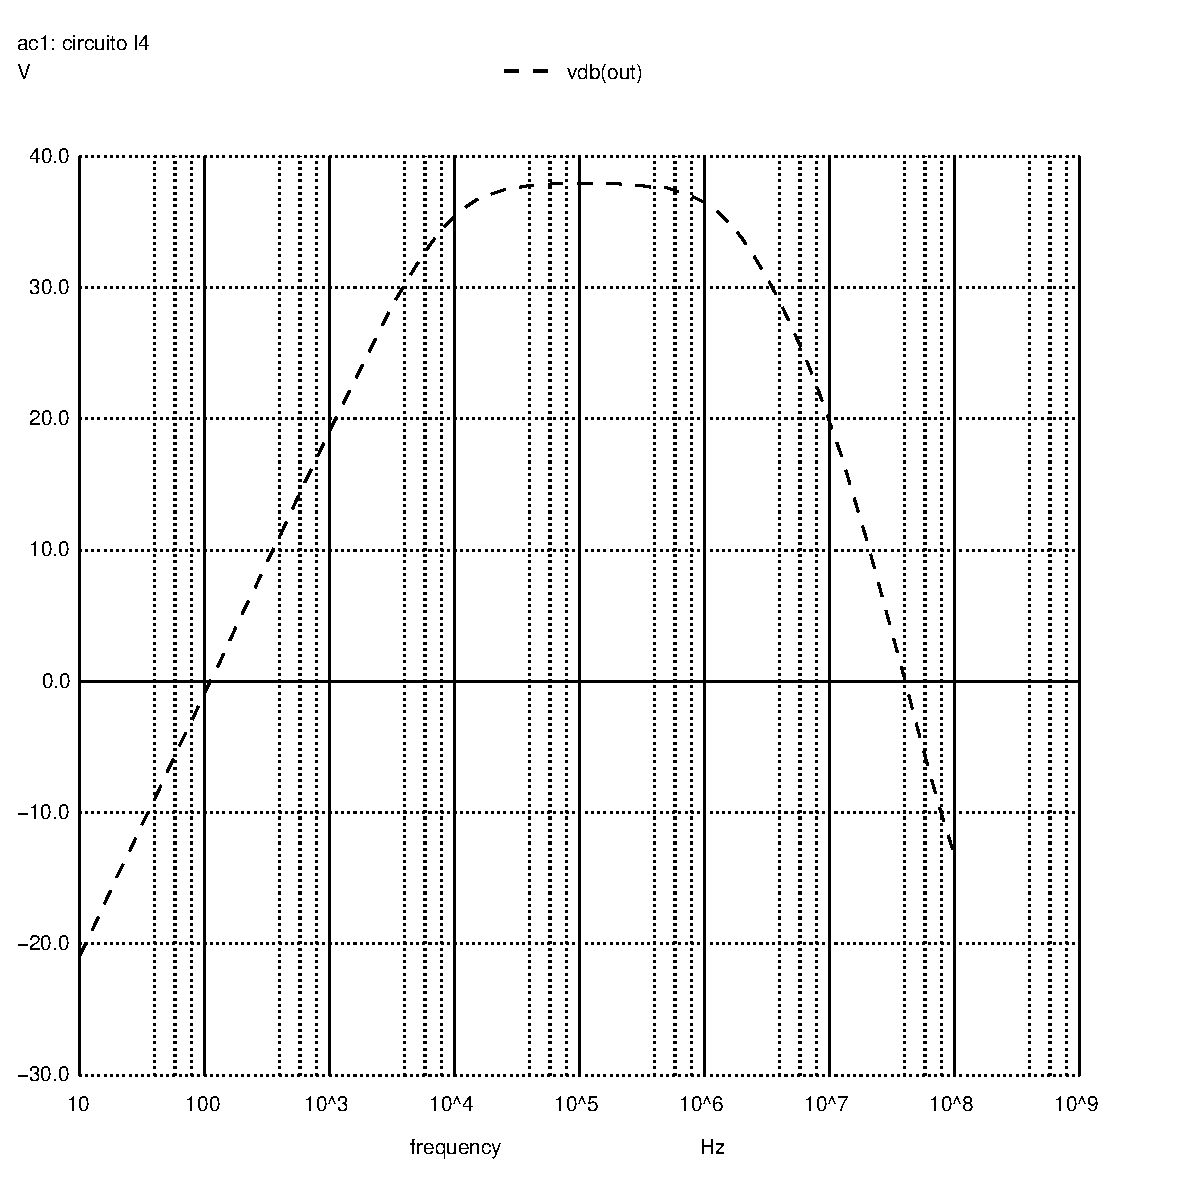
\includegraphics[scale=0.33]{images/cehigh_1.eps}
    \caption{High $C_E$ effect on Gain (1$F$)}
\end{subfigure}
\caption{$C_E$ influence}
\end{figure}

Besides that, by placing the bypass capacitor in parallel with $R_E$, this resistor becomes short for medium and high frequencies - remember the capacitor impedance is $\frac{1}{j\omega C}$. Because the amplifier's first stage gain is inversely dependent on this resistance, the bypass capacitor plays an extremelly important role in maximizing the gain for medium and high frequencies.

\subsubsection{$R_C$}

Finally, it is relevant to analyse the influence of $R_C$ on the total Gain of the circuit. 

We also present assymptotical situations in order to fully understand that behaviour.

\begin{figure}[h]
\centering
\begin{subfigure}{.5\textwidth}
    \centering
    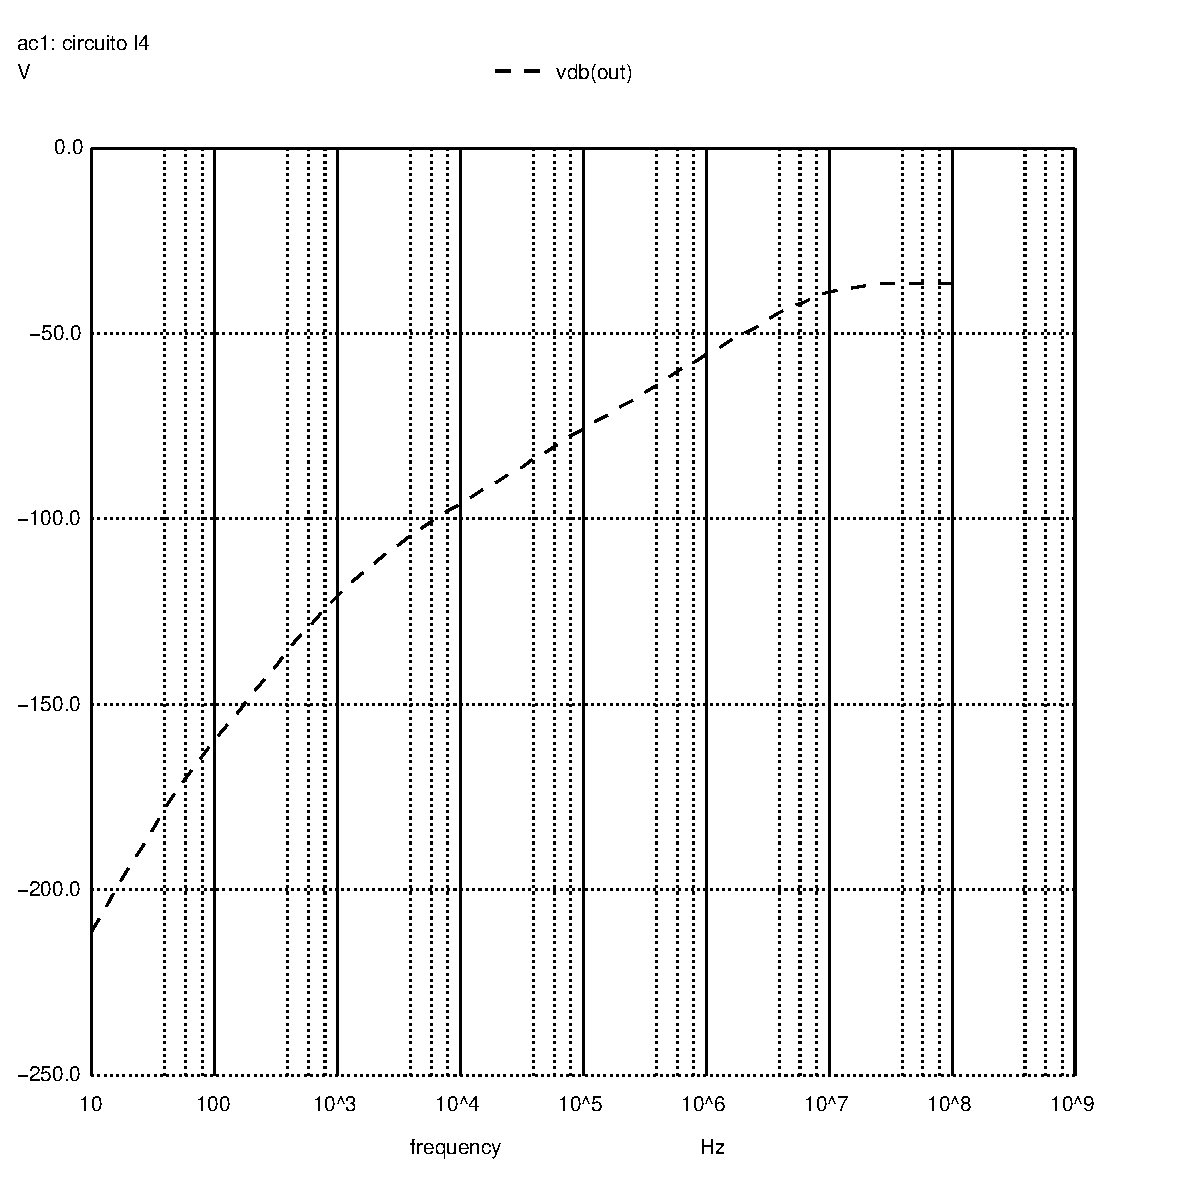
\includegraphics[scale=0.33]{images/rclow_10.eps}
    \caption{Low $R_C$ effect (on the Gain) (10$\Omega$)}
\end{subfigure}%
\begin{subfigure}{.5\textwidth}
    \centering
    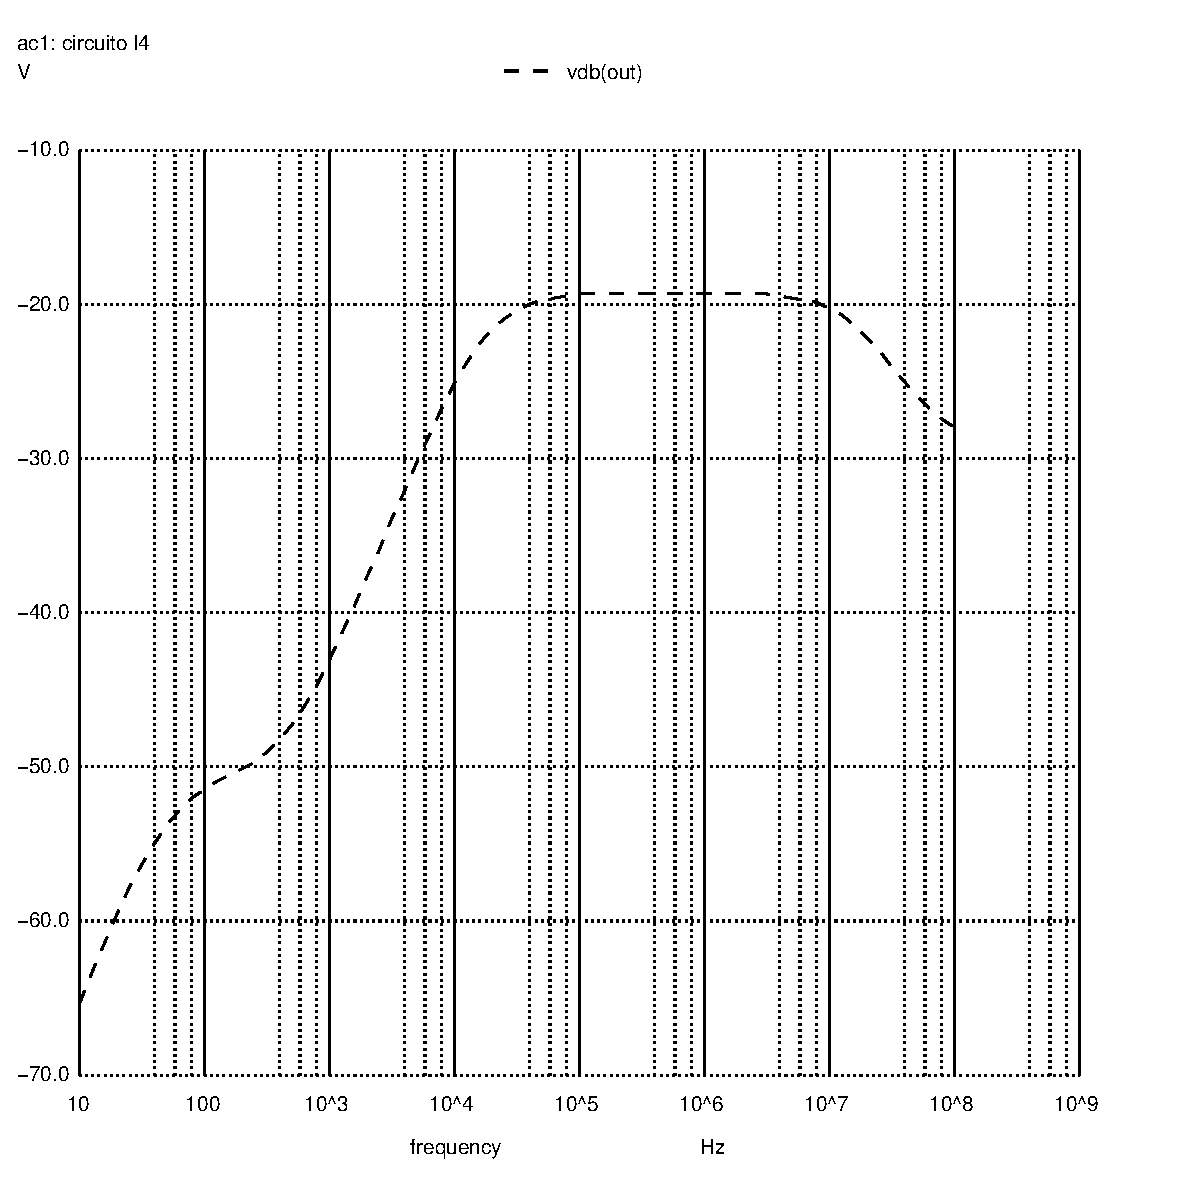
\includegraphics[scale=0.33]{images/rchigh_100k.eps}
    \caption{High $R_C$ effect on Gain (10$k\Omega$)}
    \label{fig:RC_High}
\end{subfigure}
\caption{$R_C$ influence (on the Gain)}
\end{figure}


As one can see, not only the gain increases with $R_C$ but also \textit{antecipates} the passband. This behaviour was already previewed by the theorectical anlysis on the gain, as it is proportional to $R_C$. Note that for extremely large resistance, a bizarre and slightly unpredictable behaviour occurs. 

Moreover, it is important, in order to guarantee a high compatibility with AUDIO IN and speakers, to simulate the input and output impedances of the circuit. This good compatibility is ensured with a very high input impedance ($Z_I$) and a very low output impedance ($Z_O$).  The simulation results are expressed in the following tables:

\begin{table}[h]
    \centering
    \begin{tabular}{|l|c|}
    \hline
    {\bf Name} & {\bf Value [$\Omega$]} \\ \hline
    in_imp & -563.853 + 84.4302 j\\ \hline

    \end{tabular}
    \caption{Simulation Input Impedance}
    \label{tab:simulation_input_imp}
\end{table}

\begin{table}[h]
    \centering
    \begin{tabular}{|l|c|}
    \hline
    {\bf Name} & {\bf Value [$\Omega$]} \\ \hline
    out_imp & 10.0554 + -1.18427 j\\ \hline

    \end{tabular}
    \caption{Simulation Output Impedance}
    \label{tab:simulation_output_imp}
\end{table}

As with the theoretical analysis, this simulation also gives off a slightly high output inpedance (which should ideally be lower than the load's 8 $\Omega$). As stated this fact results from the compromise needed for the merit figure.
\pagebreak

\subsection{Comparison}
\label{subsec:comparison}

We are now ready to make a global comparison of the two approaches, with the chosen values for the constants. Below, we present both the theoretical and simulation graphs of the gain:

\vspace{-2.5cm}

\begin{figure}[h]
\centering
\begin{subfigure}{.5\textwidth}
    \centering
    \vspace{2.8 cm}
    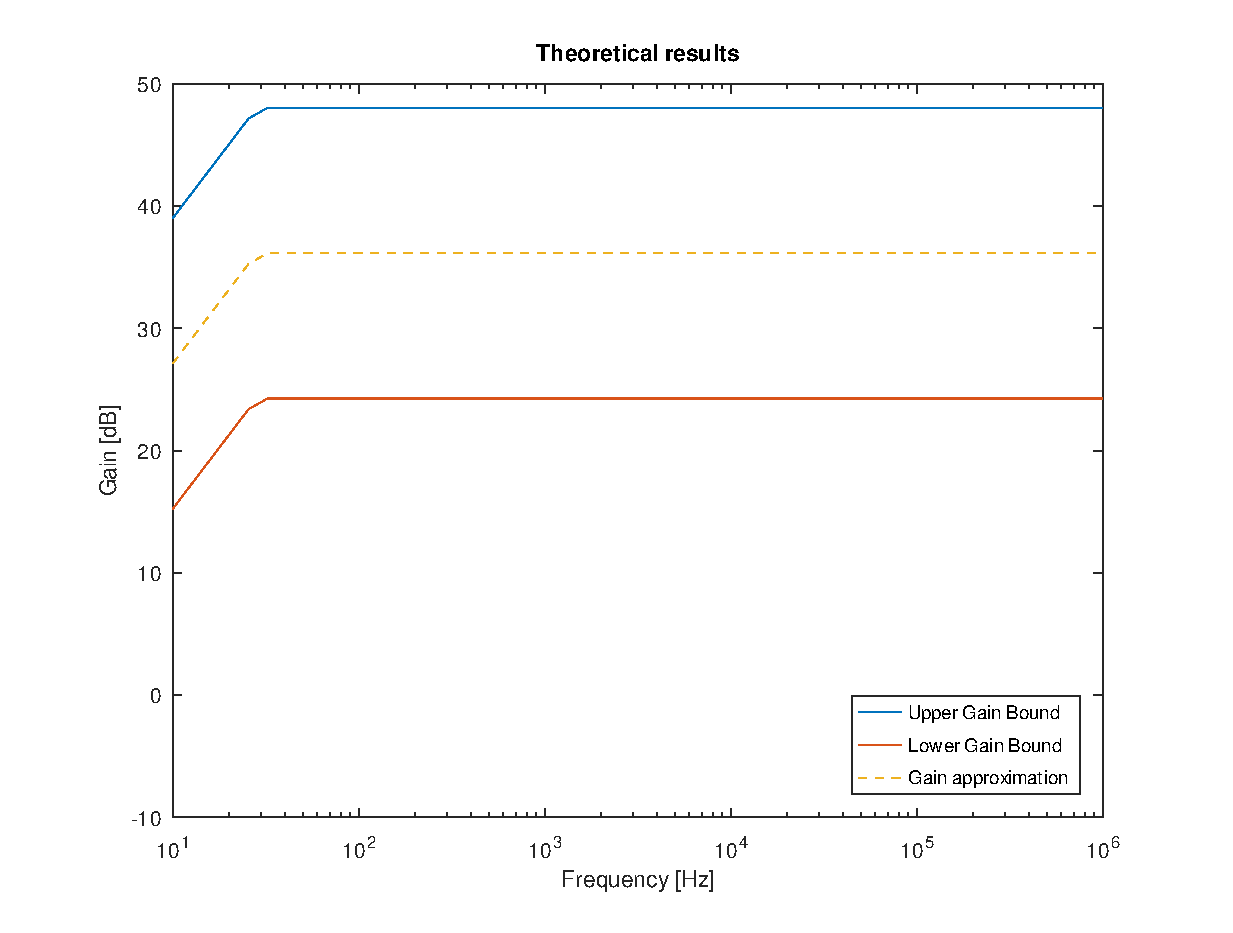
\includegraphics[scale=0.4]{theo_results.eps}
    \caption{Theoretical Gain}
\end{subfigure}%
\begin{subfigure}{.5\textwidth}
    \centering
    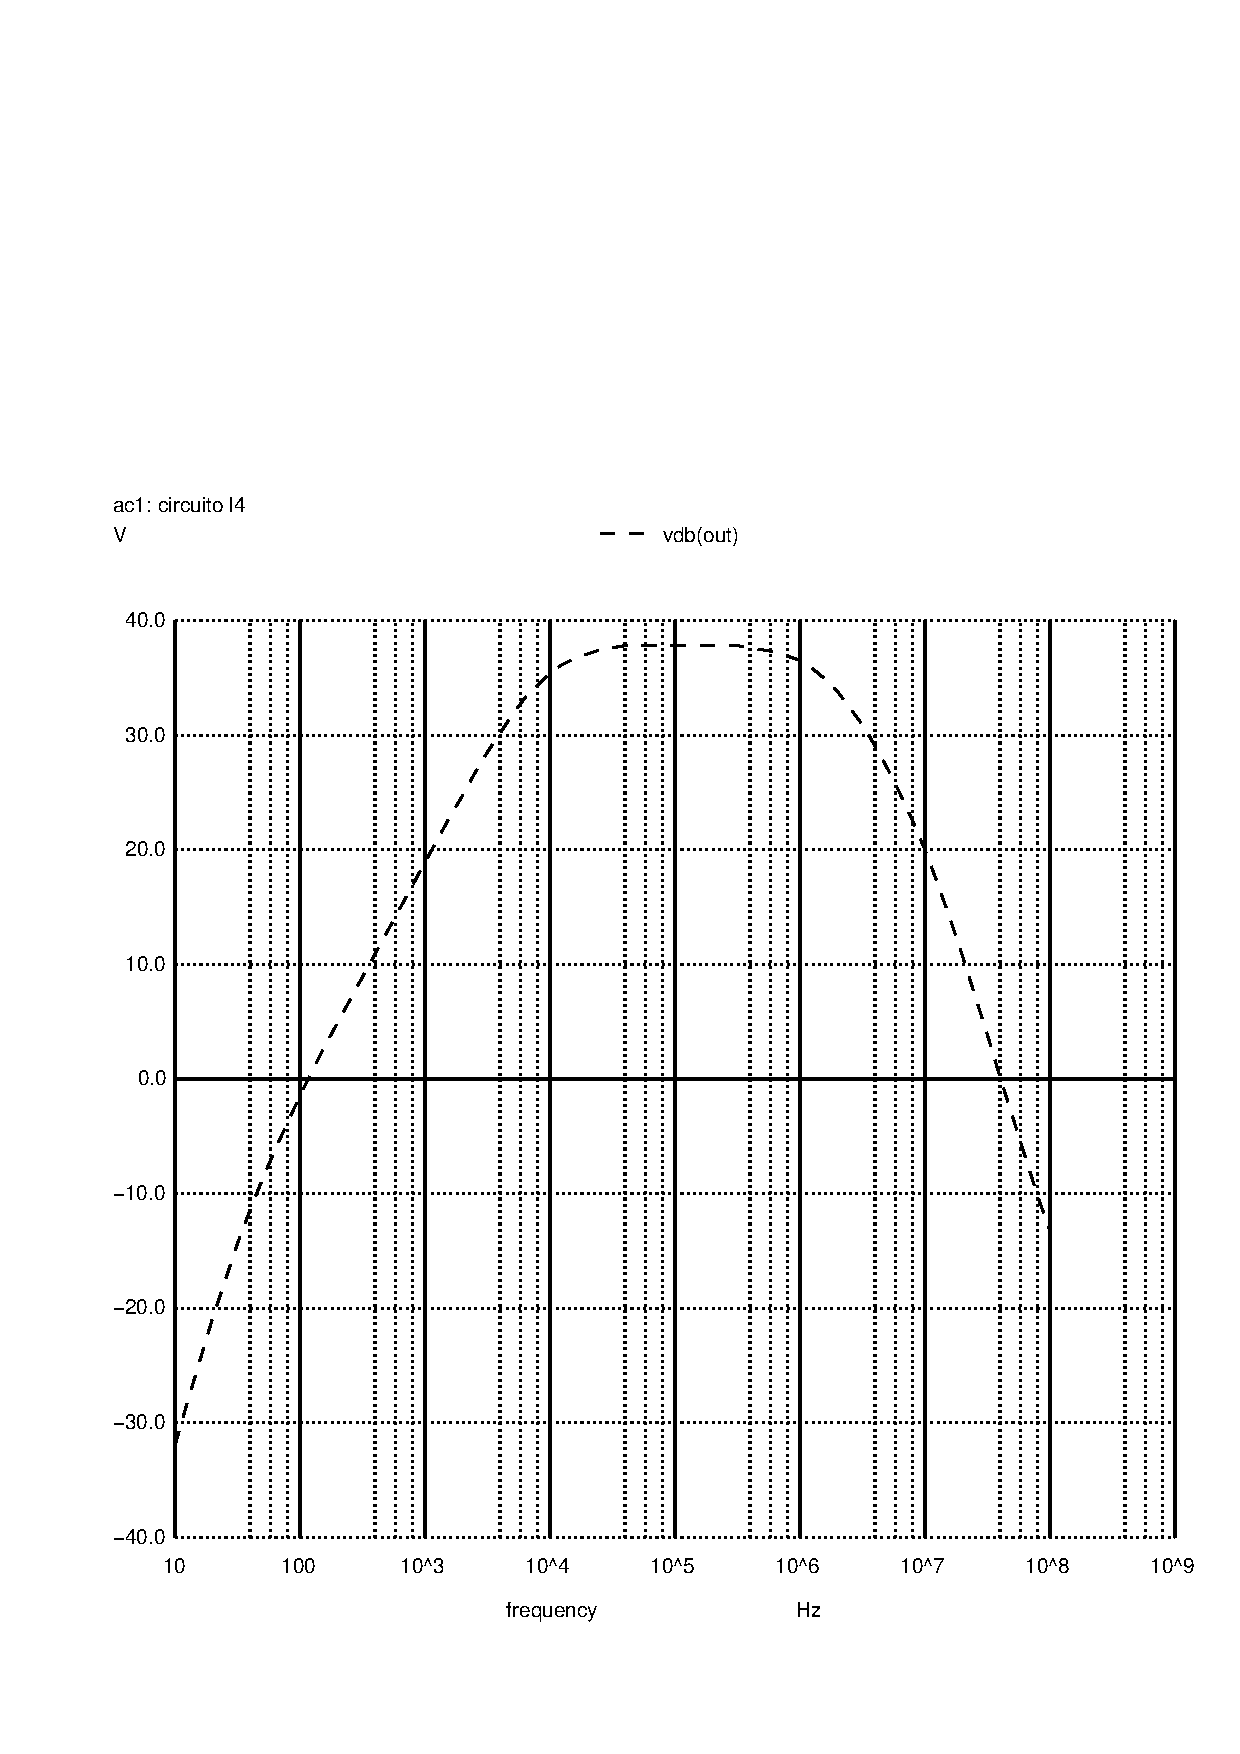
\includegraphics[scale=0.33]{vo2f.pdf}
    \caption{Simulation Gain}
\end{subfigure}
\caption{Gain}
\label{fig:Gain}
\end{figure}

In this case, the comparison of the shape can only be done on the left side, since we don't have the theoretical higher cut-off frequency. For this reason, there's no point in plotting the theoretical gain any further than $1 MHz$.

One should bear in mind that the theorectical analysis either considers the capacitors are short-circuited or are open-circuited (this approximation is made when for this analysis, the value of $R_E$ is either $0$ or $R_E$ in Table \ref{tab:constants}, respectively). For this reason, two estimates were made (Figure \ref{fig:Gain}) - in blue the capacitors are considered short-circuited; in orange the capacitors are considered open-circuited; in yellow dashed it is represented the medium-value plot, that can be considered as a rough approximation of the real gain. This theorectical approach does not guarantee a specific value for the overall gain, however it gives us a region of acceptable gains. The simulation gain obtained is satisfyingly in this prediction region. 

The overall shape of the graphs is similar, noting that the theoretical one can be thought of as assymptotical rather than a precise approach. In fact, as we imposed its shape, accordingly to the one given by \textit{Ngspice}, it is not sensible to variations that might occur (as the appearance of a \textit{second step} in \ref{fig:RC_High}).

In a greater detail analysis, when remembering the values presented in the previous subsections - $Z_I$ and $Z_O$, $A_v$ and $f_{CO_L}$ -, despite the obvious differences, the comparison is satisfactory. Comparing the order of magnitude, when putting values side by side, they are within reasonable intervals of similarity. In fact, the lower cut-off frequencies (from tables \ref{tab:theo_CO_freq} and \ref{tab:sim_results}) are really close, especially when you remember they are to be plotted in a logscale graph.

In conclusion, the theoretical approach gives a rough perspective of the overall work conditions of the amplifier, which is good in a first \textit{sketch}.

\section{Merit Results}
\label{sec:merit}

From the results obtained through the Ngspice simulation (see Section \ref{subsec:comparison}) and considering we used the data shown in Section \ref{sec:introduction}, we can compute the price and the merit using the \textit{formulae} given in the lab assignment:

\begin{table}[h]
    \centering
    \begin{tabular}{|l|c|}
    \hline
    {\bf Name} & {\bf Value} \\ \hline
    price & 2102.51\\ \hline
merit & 3.23771\\ \hline

    \end{tabular}
    \caption{Total Price and Merit}
    \label{tab:price_merit}
\end{table}

For our strategy, we opted to firstly understand what each component would produce when its values changed dramatically . So we analysed the circuit \textit{assymptotically} in order to acquire a bigger picture of the influence of each component.

After understanding that, we then made small adjustments to further perfect our results, which in turn made the merit figure rise. In this approach, we left the cost as a second thought.   

To conclude, we began decreasing the cost until we found out the perfect compromise for us, giving the results shown in table \ref{tab:price_merit}.


